\documentclass[border=6pt]{standalone}
% Shared style for the methodology figures, after the block diagrams of
% "Attention Is All You Need": rounded blocks in soft colours with fine outlines,
% a grey container with a repetition count, and thin arrows.
\usepackage{libertinus}
\usepackage{amsmath}
\usepackage{xcolor}
\usepackage{tikz}
\usetikzlibrary{positioning,arrows.meta,calc,fit,backgrounds,shapes.geometric}

\definecolor{ink}{HTML}{1E2227}
\definecolor{muted}{HTML}{5C6670}
\definecolor{cRGB}{HTML}{2F6DB5}
\definecolor{cIR}{HTML}{C0622B}
\definecolor{cFuse}{HTML}{3B8B66}
\definecolor{cTime}{HTML}{7450A8}
\definecolor{cNeutral}{HTML}{66707B}
\definecolor{cData}{HTML}{8C6A2F}
\definecolor{cAlert}{HTML}{A8384A}
\definecolor{cHead}{HTML}{B08A2E}
\color{ink}

\tikzset{
  blk/.style   = {rounded corners=3pt, align=center, font=\small, inner xsep=6pt, inner ysep=4.5pt,
                  minimum height=0.8cm, line width=0.5pt, text=ink,
                  execute at begin node={\hyphenpenalty=10000}},
  vis/.style   = {blk, fill=cRGB!14, draw=cRGB!65},
  thr/.style   = {blk, fill=cIR!15, draw=cIR!65},
  fus/.style   = {blk, fill=cFuse!16, draw=cFuse!70},
  scn/.style   = {blk, fill=cTime!14, draw=cTime!65},
  neu/.style   = {blk, fill=cNeutral!10, draw=cNeutral!55},
  hed/.style   = {blk, fill=cHead!16, draw=cHead!70},
  dat/.style   = {blk, fill=cData!12, draw=cData!60},
  io/.style    = {align=center, font=\small, text=ink},
  op/.style    = {circle, draw=cNeutral!70, fill=white, line width=0.5pt, inner sep=0pt,
                  minimum size=5.2mm, font=\small},
  lab/.style   = {font=\footnotesize\itshape, text=muted, align=center},
  note/.style  = {font=\footnotesize, text=muted, align=left},
  ar/.style    = {-{Stealth[length=2.1mm,width=1.6mm]}, line width=0.55pt, draw=ink!75},
  dar/.style   = {ar, dash pattern=on 2.4pt off 1.6pt},
  gar/.style   = {ar, draw=cData, dash pattern=on 2.4pt off 1.6pt},
  box/.style   = {rounded corners=6pt, fill=cNeutral!5, draw=cNeutral!45, line width=0.5pt},
  over/.style  = {preaction={draw=white, line width=3.2pt, -}},
}

\begin{document}
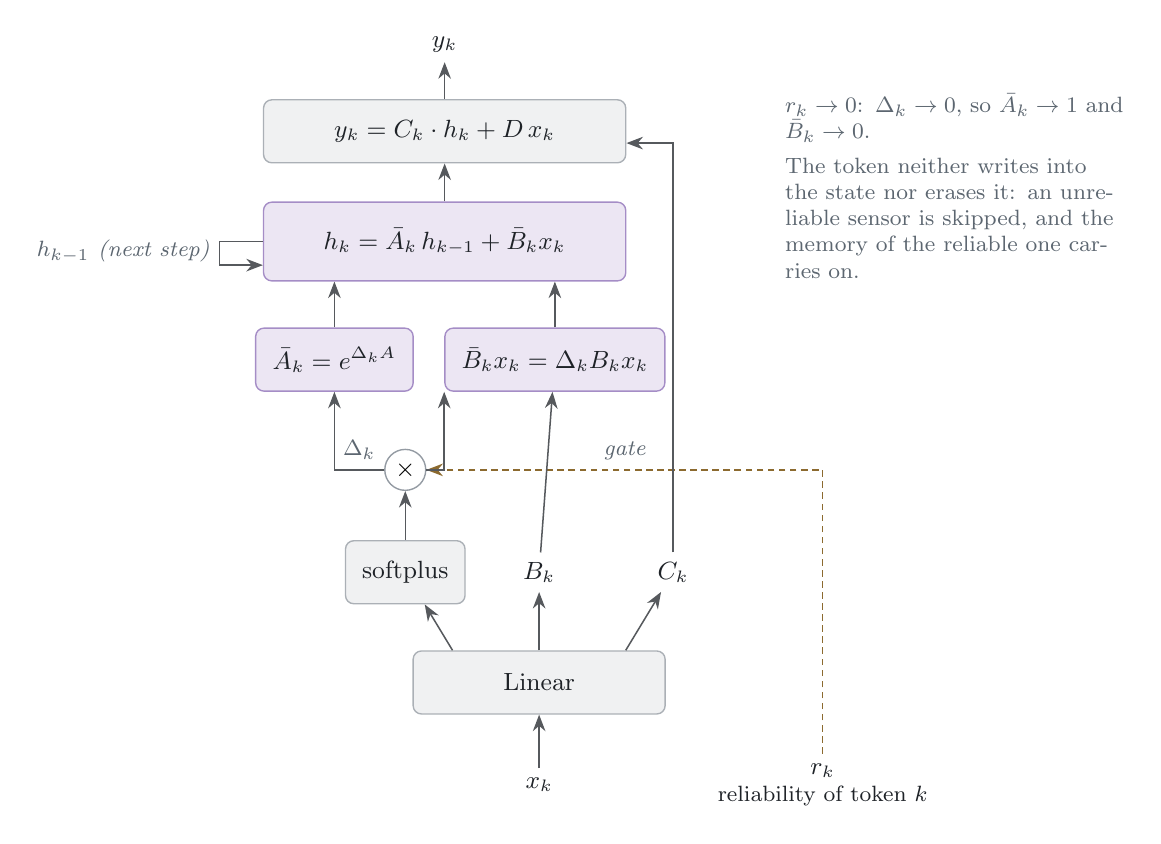
\begin{tikzpicture}
  \node[io] (x) at (0,0) {$x_k$};
  \node[io] (r) at (3.6,0) {$r_k$\\[-1pt] \footnotesize reliability of token $k$};

  \node[neu, minimum width=3.2cm] (lin) at (0,1.3) {Linear};
  \draw[ar] (x) -- (lin);

  \node[neu, minimum width=1.4cm] (sp) at (-1.7,2.7) {softplus};
  \node[io] (B) at (0,2.7) {$B_k$};
  \node[io] (C) at (1.7,2.7) {$C_k$};
  \draw[ar] ($(lin.north)+(-1.1,0)$) -- (sp);
  \draw[ar] (lin) -- (B);
  \draw[ar] ($(lin.north)+(1.1,0)$) -- (C);

  \node[op] (mul) at (-1.7,4.0) {$\times$};
  \draw[ar] (sp) -- (mul);
  \draw[gar] (r) |- (mul.east) node[pos=0.75, lab, above] {gate};

  \node[scn, minimum width=2.0cm] (dA) at (-2.6,5.4) {$\bar A_k = e^{\Delta_k A}$};
  \node[scn, minimum width=2.2cm] (dB) at (0.2,5.4) {$\bar B_k x_k = \Delta_k B_k x_k$};
  \draw[ar] (mul) -| node[lab, pos=0.25, above] {$\Delta_k$} (dA);
  \draw[ar] (mul) -| (dB.south west);
  \draw[ar] (B) -- (dB);

  \node[scn, minimum width=4.6cm, minimum height=1.0cm] (h) at (-1.2,6.9) {$h_k = \bar A_k\, h_{k-1} + \bar B_k x_k$};
  \draw[ar] (dA) -- (dA |- h.south);
  \draw[ar] (dB) -- (dB |- h.south);
  \draw[ar] (h.west) -- ++(-0.55,0) |- node[lab, pos=0.2, left] {$h_{k-1}$ (next step)} ($(h.west)+(0,-0.3)$);

  \node[neu, minimum width=4.6cm] (y) at (-1.2,8.3) {$y_k = C_k \cdot h_k + D\,x_k$};
  \draw[ar] (h) -- (y);
  \draw[ar] (C) |- ($(y.east)+(0,-0.15)$);
  \node[io] (out) at (-1.2,9.4) {$y_k$};
  \draw[ar] (y) -- (out);

  \node[note, anchor=north west, text width=4.3cm] at (3.0,8.9)
    {$r_k \to 0$: $\Delta_k \to 0$, so $\bar A_k \to 1$ and $\bar B_k \to 0$.\\[3pt]
     The token neither writes into the state nor erases it: an unreliable sensor is skipped, and the memory of
     the reliable one carries on.};
\end{tikzpicture}
\end{document}
